\chapter{Massive corpus summarisation}

In this chapter we present novel submodular functions that can be applied to
find the most important documents out of millions of interconnected documents
such as parts of the web (or even the whole web).
Our approach expands on the ideas of \emph{multi-document summarisation using
submodular word coverage} \cite{sipos2012temporal} presented in
Chapter~\vref{cap:submodularity}.
This chapter presents the authors' novel contributions to the problem of
\emph{massive corpus summarisation}.

\section{Scaling from thousands to millions}

Sipos et al \cite{sipos2012temporal} present an interesting way to summarise a
document corpus using \emph{submodular functions}. However, their focus is on
the different ways one can view summarisation and their methods are hard or
even impossible to scale beyond tens of thousand of documents.
In this thesis we concentrate on finding the most important articles out of a
massive corpus of interconnected documents. This can be viewed as a
multi-document summarisation task, but given the small ratio between the
number of selected documents and the total size of the corpus it also bears
some differences from the classical view on multi-document summarisation.
Concretely, we aim to select tens of \emph{Wikipedia} articles from about
\(1.3\) million \emph{Wikipedia} pages\footnote{This is the total number of
human-written articles in \emph{Wikipedia} before Oct 2012}.

This problem is two-folded. On one hand, we have to adapt the submodular
functions so that they yield satisfying results for such a large
\emph{'compression' ratio} of about \(1/50000\) (as it is in the case of
Wikipedia). On other hand, we can no longer run sequentially; so, in turn, we
will employ having all algorithms written in a \emph{MapReduce}
\cite{dean2008mapreduce} distributed fashion. If you are interested in more
details about the framework we implemented please refer to
Chapter~\vref{cap:wikimining}.

\section{Scaling influential documents}
\label{sec:scale-doc-influence}

In Section~\vref{sec:doc-influence} we described the \emph{document influence}
function proposed in \cite{sipos2012temporal}.
While we can apply the function as it is to small corpora (up to a couple tens
of thousands documents), in order to make it scale to Wikipedia's size --
around 1.3 million human-written articles -- we have to make changes to part of
the submodular function.

Most of the general issues we had to solve are conceptual or engineering
problems, such as:
\begin{enumerate}
  \item finding a suitable \emph{creation date / year};
  \item finding the k-nearest neighbours for each document;
  \item computing the two component functions:
  \begin{itemize}
    \item \(\theta(w, y)\) -- word spread.
    \item \(\nu(d, w)\) -- document novelty;
  \end{itemize}
\end{enumerate}

\paragraph{Creation date}
To find a suitable \emph{creation date} in the case of web pages (more
specifically, Wikipedia pages) is a much harder task than to finding the
publishing date of a paper.
In the case of Wikipedia we settled on using the \emph{last modified date} as
an imperfect measure of creation date. A better approach is to find the most
important revision and use that as the page's creation date \footnote{For more
details about future work, see Section~\vref{sec:future-work}}.

\paragraph{K-nearest-neighbours}
Given the massive size of the corpora, we cannot use \ac{kNN} to compute the
nearest neighbours. As a result, we employed using \ac{LSH} to approximately
compute the 1-nearest neighbour of each page. The authors in
\cite{sipos2012temporal} observe -- in their experimental results -- that
selecting only one neighbour is sufficient for the purposes of this submodular
function. Furthermore, using \ac{LSH} instead of an exact \ac{kNN} approach
does not influence our results either.

\paragraph{Component functions}
As a result of the tf-idf matrix size, computing the two functions -- \(\nu(d,
w)\) and \(\theta(w, y)\) -- has to be done in separate \aclp{MR} as part of
the \emph{preprocessing} steps The same holds true for retrieving the creation
date of each article.

\section{Graph coverage}
\label{sec:graph-coverage}

In this section we present a submodular function defined on the \emph{inlinks}
graph structure of the considered set of documents. Instead of only evaluating
the selected document we argue that each node expands its influence among its
neighbouring articles.

\subsection{Definition}

\begin{definition}[Graph coverage]
  \label{def:graph-coverage}
  Let \(G = (D, E)\) be a graph where:
  \begin{align*}
    D &:= \text{set of document vertices,} \\
    E &:= \text{set of edges.}
  \end{align*}
  Then we define:
  \begin{align*}
    &f : 2^D \to \R_+ \\
    &f(S) := |\bigcup_{d \in S} V_d|
  \end{align*}
  where:
    \[V_d := \{d\} \cup \{v \in D | (v, d) \in E\} \text{.}\]
\end{definition}

\begin{proposition}
  \label{prop:graph-coverage}
  Graph coverage from Definition~\ref{def:graph-coverage} is monotone
  submodular.
  \begin{proof}
    Easily proven as it can be reduced to the coverage function presented in
    Definition~\vref{def:set-coverage}.
  \end{proof}
\end{proposition}

In Figure~\ref{fig:graph-cov} we offer a visual representation of this function.
\begin{figure}
  \centering
  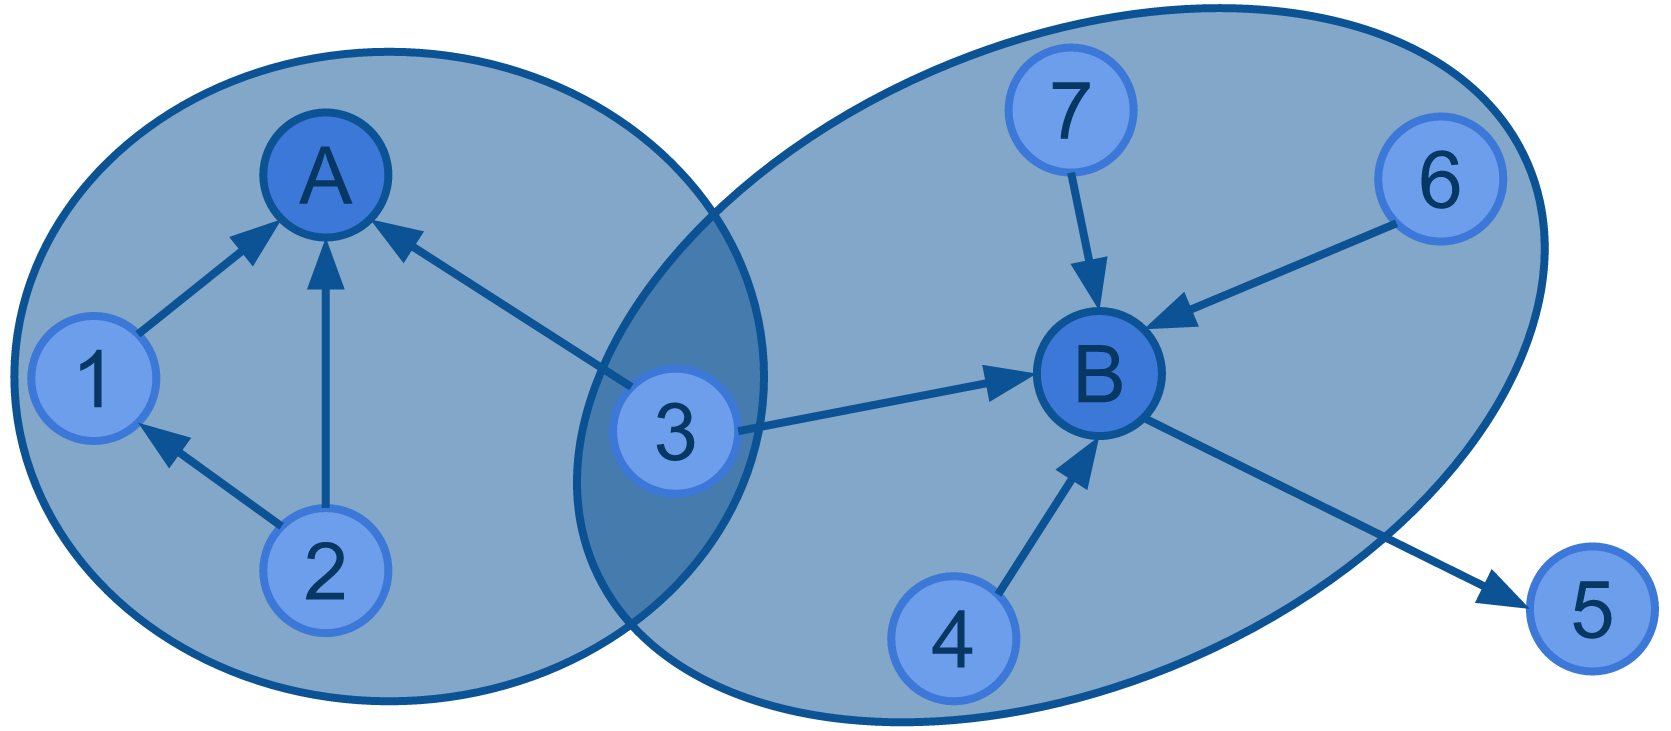
\includegraphics[width=0.9\textwidth,natwidth=1671,natheight=731]{images/graph-cov.png}
  \caption{Visual representation of \emph{graph coverage} submodular function.}
  \label{fig:graph-cov}
\end{figure}

\subsection{Rationale}

Graph coverage is a simple function that aims to measure a document's coverage
in terms of vertices it covers, while keeping the selected documents
diversified.
We argue that each document manifest an aura of influence among the articles
that link to it.
Consequently, we conjecture that adding the source document -- the page
that adds the highest number of new inlinks -- captures a topic that is both
important and sufficiently different from the already selected articles.
As a simple extension, Definition~\vref{def:graph-coverage} can be modified to
consider neighbours at a radius larger than one (for example, to take into
account all nodes that are at most two edges away from the selected document).

\section{LSH buckets}
\label{sec:lsh-buckets}

In this section we present a submodular function defined on the buckets that
result from applying \acl{LSH} to the documents' tf-idf vectors. This function
aims to increase the topic diversity of selected documents by selecting
articles that cover multiple different buckets.

\subsection{Definition}

\begin{definition}[\ac{LSH} buckets]
  \label{def:lsh-buckets}
  Let:
  \begin{align*}
    &D := \text{ set of documents,} \\
    &\B
    \begin{aligned}[t]
      :&= \{B_i \subseteq D | B_i := \ac{LSH} \text{ bucket } i\}.
      &= \{B_1, B_2, \ldots, B_b\} \\
    \end{aligned}
  \end{align*}
  Then we define:
  \begin{align*}
    &f : 2^D \to \R_+ \\
    &f(S) := \sum_{i=1}^b |B_i| \cdot g(|S \cap B_i|),
  \end{align*}
  where:
    \[g : \N \to \R_+ \text{ is concave.}\]
\end{definition}

\begin{proposition}
  \label{prop:lsh-buckets}
  \ac{LSH} buckets from Definition~\ref{def:lsh-buckets} is monotone
  submodular.
  \begin{proof}
    Easily provable using the properties of submodular functions
    \cite{krause2012submodular}.
  \end{proof}
\end{proposition}

In Figure~\ref{fig:lsh-buckets} we offer a visual representation of this
function.
\begin{figure}
  \centering
  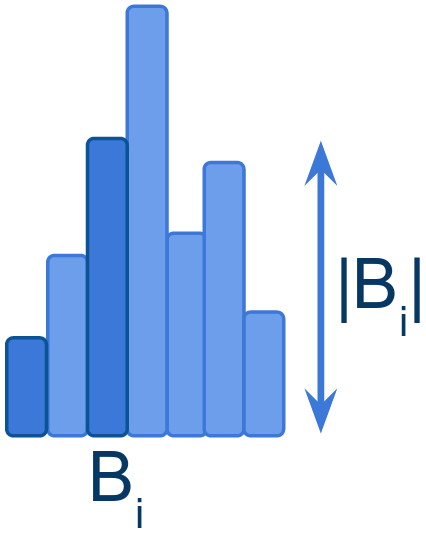
\includegraphics[width=0.3\textwidth,natwidth=426,natheight=535]{images/lsh-buckets.png}
  \caption{Visual representation of \emph{LSH buckets} submodular function.}
  \label{fig:lsh-buckets}
\end{figure}

\subsection{Rationale}

\ac{LSH} buckets is a simple function designed to be combined with other
submodular functions. The idea behind this function is that buckets group
similar documents together (using a measure such as cosine similarity, for
example).

In this regard, buckets that have more articles represent denser clusters of
pages, which we argue they define an important area or field.
As a consequence we give higher importance -- a higher weight -- to dense
buckets, multiplying by the size of the bucket: term \(|B_i|\).
On the other hand, we also value documents that are in multiple buckets: term
\(|S \cap B_i|\).
Ideally, these pages cover more than one topic and, as such, are an important
source of information if they are part of the summary.

Describing the function as a whole, our objective is to have diversity by
picking pages from different buckets while gauging both the importance of a
bucket and the topic coverage of the articles themselves.

\section{Beyond word coverage}
\label{sec:word-coverage++}

In Section~\vref{sec:word-coverage} we introduced \emph{word coverage} as a
measure of information coverage based on words that tries to avoid eccentric
documents.
However, as you can see from our results in Chapter~\vref{cap:experiments},
\emph{word coverage} performs poorer than expected when scaled to
\emph{Wikipedia}'s size (millions of documents).
In this, chapter we modify the function such that it takes into account more
information about documents when comparing them.

\subsection{Definitions}

We remind the reader that in Definition~\vref{def:word-coverage} we described a
submodular function that uses word coverage as follows:
\begin{align*}
  &f : 2^D \to \R_+
  &f(S) := \sum_{w \in W} \theta(w) \max_{d \in S} \phi(d, w)
  \,(\forall S \subseteq D)
\end{align*}
For details about the notations used we advise the reader to return to
Definition~\vref{def:word-coverage}.

In this section we propose explicit definitions for functions \(\theta(w)\) and
\(\phi(d, w\) such that they yield desirable results even for large-scale
corpora.
Let:
\begin{align*}
  D &:= \text{set of documents,} \\
  W &:= \text{set of all words from all documents in \(D\),} \\
  (D, E) = G &:= \text{ documents' graph.}
\end{align*}

\subsubsection{Word importance}

Word importance is the weight we give to a word in terms of its meaning. As we
mentioned before, there has been significant work done on how to properly
define it \cite{sipos2012temporal} \cite{lin2010multi} \cite{sipos2012large}.
Here we use some of the basic metrics such that it easily scales to a massive
corpus.

\begin{definition}[Word importance]
  \label{def:word-importance}
  We define word importance
  \[\theta : W \to \R_+\]
  in one of the following four (non-equivalent) ways:
  \begin{enumerate}
    \item \(\theta(w) := \sqrt{wc(w)}\)
    \item \(\theta(w) := \ln(wc(w))\)
    \item \(\theta(w) := \sqrt{dc(w)}\)
    \item \(\theta(w) := \ln(dc(w))\)
  \end{enumerate}
  where:
  \[\text{wc, dc} : W \to \R_+\]
  \begin{align*}
    wc(w) &:= \sum_{d \in D} count(w, d), \\
    count(w, d) &:= \text{number of times word \(w\) appears in document
      \(d\),} \\
    dc(w) &:= |\{w \in d | d \in D\}|.
  \end{align*}
\end{definition}
Functions \(wc(w)\) and \(dc(w)\) are functions needed to define tf-idf
\cite{salton1988term}:
\begin{itemize}
  \item \(wc(w)\) stands for \emph{word count} and
    represents the number of times word \(w\) appears in the whole corpus;
  \item \(dc(w)\) stands for \emph{document count} and represents the number of
  documents (from the corpus) in which word \(w\) appears.
\end{itemize}

\subsubsection{Coverage of a word}

The coverage of a word in a document is a measure of how much a word covers a
specific concept in that document. In our case we view the coverage of a word
as the \emph{meaningfulness} of that word in a document in the context of all
other words and documents from the corpus. Here we define novel functions that
consider some of the different metrics one can use for this task.

\begin{definition}[Coverage of a word]
  \label{def:coverage-of-word}
  We define coverage of a word
  \[\phi : D \times W \to \R_+\]
  in one of the following (non-equivalent) ways:
  \begin{align*}
    \phi(d, w) = \text{tf-idf}(d, w)\, &[\cdot\, \text{\#inlinks}(d)] \\
        &[\cdot\, \text{\#revisions}(d)] \\
        &[\cdot\, \text{revisions-volume}(d)],
  \end{align*}
  where:
  \[\text{\#inlinks, revisions-volume, \#revisions} : D \to \R_+\]
  \begin{align*}
    \text{\#inlinks}(d) &:= |\{v \in D | (v, d) \in E\}|, \\
    \text{\#revisions}(d) &:= \text{number of edits of document } d, \\
    \text{revisions-volume}(d) &:= \text{total size of edits of document } d.
  \end{align*}
  Note that \([\cdot]\) marks an optional term. As such we get twelve different
  possible functions in total.
\end{definition}
Also note that using any explicit forms for \emph{word importance} from
Definition~\ref{def:word-importance} and for \emph{coverage of a word} from
Definition~\ref{def:coverage-of-word} maintains the \emph{word coverage}
function from Definition~\vref{def:word-coverage} \emph{monotone submodular}.

\subsection{Rationale}

We were unsatisfied with the results of using only tf-idf for the
\emph{coverage of a word in a document}, so we thought about natural ways to
extend \(\phi(d, w)\) to capture more of the available information.
One of the main problems was that although we take into account the \emph{word
importance} in Definition~\ref{def:word-coverage} this is not enough to dampen
the eccentricity of the articles.
In the following paragraphs we explain how each added term from
Definition~\ref{def:coverage-of-word} fits in and what is the reasoning behind
it.
We warn the reader that we offer only intuitive explanations that were
empirically confirmed, but no strict formalisms about their validity.

\subsubsection{Inlinks}

The idea for inlinks has two justifications behind it that are similar, but
distinct concepts.

One of them is merging \emph{graph coverage} presented in
Section~\ref{sec:graph-coverage} with \emph{word coverage}.
This can be achieved, and we present the way it can be done it
Section~\ref{sec:combine}, but we could not find appropriate parameters to use
that approach.

The other is seeing inlinks as a citations measure.
This has been used somewhat successfully in web ranking and it has since
evolved into \emph{PageRank} and other more sophisticated, hybrid approaches,
but here we are using it in its plain form viewing Wikipedia different from a
(competitive) game.
However, using \emph{PageRank} or more advanced measure might prove to be a
useful tweak to our current approach.

\subsubsection{Revisions}

While our goal is to find time-agnostic important articles, and as such we
would like to stay away from transitional popular articles, we consider that
adding a measure of \emph{popularity} and/or \emph{controversy} into our
functions improves our results considerably.

While combining \emph{number of revisions} and \emph{revision volume} - total
size of all revisions of an articles - together is validated entirely in an
empiric fashion, through experiments, each individual term has a interpretation
behind it.

\paragraph{Number of revisions}
We can view \emph{number of revisions} as a foremost \emph{controversy} measure
as articles with high edit count were changed a lot of times (by different
persons); this means there existed different users with diverging opinions on
the given topic. For example, this can happen in case of a celebrities death.

\paragraph{Revision volume}
On the other side, we can interpret \emph{revision volume} as a measure of
popular interest. Articles with high revision volumes have both a sizeable
length and a considerable percentage of big changes made by users passionate
about the given topic.

\section{Combining multiple submodular functions}
\label{sec:combine}

In Section~\vref{sec:submod-functions} we mentioned
Proposition~\ref{prop:linear-combinations} that allows us to combine multiple
submodular functions together.
However, there are two main problems that arise:
\begin{enumerate}
  \item choosing the \(\lambda_i\) parameters.
  \item the functions have to be of the same magnitude -- ideally even grow
  similarly;
\end{enumerate}

For the first problem we empirically try different hand-picked combinations.
While there is an entire field of \ac{ML} that deals with \emph{parameter
selection} we considered this to be outside the scope of this thesis.
For the second problem, we present our solution in the next subsection.

\subsection{Normalisation}

Here we present a way to normalize the functions we defined in the sections
above, so that one can (more) easily combine them using linear combinations.
It is important to note that we can only divide the functions' expressions by
constants with respect to \(S\) so that the functions remain \emph{monotone
submodular}.

\emph{Word coverage} and \emph{document influence} are already in a good spot
because the tf-idf vectors are both normalized and very sparse and, as a
consequence, the values remain small (\(< 1\)) even when summing then together.

\paragraph{LSH buckets}
In Definition~\vref{def:graph-coverage}, we defined \emph{LSH buckets} as: \(f(S) := \sum_{i=1}^b |B_i| \cdot g(|S \cap
B_i|)\).  \(g(S \cap B_i\)) is bounded by \(g(B_i)\) and we can then take the
weighted average with respect to \(|B_i|\). This results in:
\[
  f(S) :=
    \frac{1}{\sum_{i=1}^b |B_i|} \cdot
    \sum_{i=1}^b \left[ |B_i| \cdot \frac{g(|S \cap B_i|)}{g(|B_i|)} \right]
\]
that is always \(\leq 1\).

\paragraph{Graph coverage}
In Definition~\vref{def:lsh-buckets}, we defined \emph{graph coverage} as:
\(f(S) := |\bigcup_{d \in S} V_d|\).
This function is bounded by the number of vertices (documents): \(|D|\). This
results in:
\[
  f(S) := \frac{|\bigcup_{d \in S} V_d|}{|D|}
\]
that is always \(\leq 1\).

